% !TEX root=../main.tex

\section{Semantics}
\label{sec:semantics}

In this section we discuss the symbolic execution semantics for \TOPHAT.
The structure of the symbolic semantics closely resembles that of the concrete semantics.
It consists of three layers, a big step symbolic evaluation semantics for the host language, a big step symbolic normalisation semantics for the task language, and a small step driving semantics that processes user inputs.
\Cref{fig:semantic-functions} gives an overview of the relations between the different semantics.

\begin{figure}[h]
  \centering
  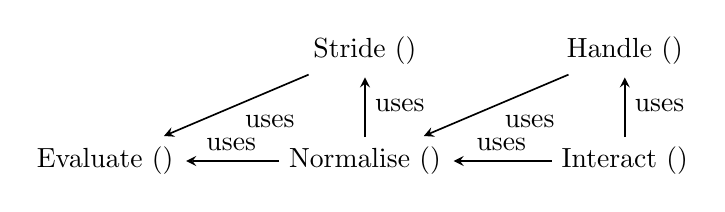
\begin{tikzpicture}[
              > = stealth, % arrow head style
              shorten > = 1pt, % don't touch arrow head to node
              auto,
              node distance = 2.3cm, % distance between nodes
              semithick, % line style
          ]

          \node (interact)  {Interact ($\siminteract$)};
          \node (handle) [above of=interact,yshift=-.9cm] {Handle ($\simhandle$)};
          \node (normalise) [left of=interact,xshift=-1cm] {Normalise ($\simnormalise$)};
          \node (stride) [left of=handle,xshift=-1cm] {Stride ($\simstride$)};
          \node (evaluate) [left of=normalise,xshift=-1cm] {Evaluate ($\simeval$)};


          \path[->,right] (interact) edge node {uses} (handle);
          \path[->,above] (interact) edge node {uses} (normalise);

          \path[->] (handle) edge node {uses} (normalise);

          \path[->,right] (normalise) edge node {uses} (stride);
          \path[->,above] (normalise) edge node {uses} (evaluate);

          \path[->] (stride) edge node {uses} (evaluate);

      \end{tikzpicture}
  \caption{
    Semantic functions defined in this report and their relation.
  }
  \label{fig:semantic-functions}
\end{figure}

They are described in the following sections.
We will study their interesting aspects, and the changes made with respect to the concrete semantics.



\subsection{Symbolic evaluation}

The host language is a simply typed lambda calculus with references and basic operations.
Most of the symbolic evaluation rules closely resemble the concrete semantics.
The original evaluation relation ($\eval$) had the form $\RelationE$,
where an expression $e$ in a state $\sigma$ evaluates to a value $v$ in state $\sigma'$.
The new relation ($\simeval$) adds path conditions $\phi$ to the output and has the form $\RelationSE$.
The tilde distinguishes the old concrete and the new symbolic variants.

The symbolic semantics can generate multiple outcomes.
This is denoted in the evaluation with a line over the result, which can be read as $\overline{\simv,\sims',\phi} = \{(\simv_1,\sims'_1,\phi_1),\cdots,(\simv_n,\sims'_n,\phi_n)\}$.
The set that results from symbolic execution can be interpreted as follows.
Each element is a possible endpoint in the execution of a task.
It is guarded by a condition $\phi$ over the symbolic input.
Execution only arrives at the symbolic value $\simv$ and symbolic state $\sims'$ when the path condition $\phi$ is satisfied.

To illustrate the difference between concrete and symbolic evaluation, \cref{fig:oldToNewSemantics} lists one rule from the concrete semantics and its corresponding symbolic counterpart.

\begin{figure}[ht]
  \small
  \begin{gather*}
    \userule{E-Edit}\Quad
    \userule{SE-Edit}
  \end{gather*}
  \caption{The evaluation rule from the concrete and the symbolic semantics for the editor expression.}
  \label{fig:oldToNewSemantics}
\end{figure}

The \refrule{E-Edit} rule evaluates the expression held in an editor to a value.
The \refrule{SE-Edit} does the same, but since it is concerned with symbolic execution, the expression can contain symbols.
We therefore do not know beforehand which concrete value will be produced, or even which path the execution will take.
If the expression contains a conditional that depends on a symbol, there can be multiple possible result values.

% Figure~\ref{fig:eval} lists the rule for conditional.
% From this rule, one can clearly see that both branches are calculated, since at this point we do not know, what the condition will evaluate to.

Most symbolic rules closely resemble their concrete counterparts, and follow directly from them.
The rules are not listed here, a full overview can be found in the appendix online \footnote{\url{https://github.com/timjs/symbolic-tophat/raw/master/appendix.pdf}}.

The only interesting rule is the one for conditionals, listed in \cref{fig:eval}.
\begin{figure}[ht]
  \small
  \begin{gather*}
    \boxed{\RelationSE} \Break
    \userule{SE-If}
  \end{gather*}
  \caption{Part of the symbolic evaluation semantics.}
  \label{fig:eval}
\end{figure}
The concrete semantics has two separate rules for the $\THEN$ and the $\ELSE$ branch.
The symbolic semantics has one combined rule \refrule{SE-If}.
Since $\sime_1$ can contain symbols, it can evaluate to multiple values.
The rule keeps track of all options.
It calculates the $\THEN$-branch, and records in the path condition that execution can only reach this branch if $\simv_1$ becomes $\True$.
The rule does the same for the $\ELSE$-branch, except it requires that $\simv_1$ becomes $\False$.
Note that both $\sime_2$ and $\sime_3$ are evaluated using the same state $\sims'$,
which is the resulting state after evaluating $\sime_1$.



\subsection{Observations}
\label{subsec:observations}

The symbolic normalisation and driving semantics make use of observations on tasks, just like the concrete semantics.

The partial function $\Value$ can be used to observe the value of a task.
Its definition is given in \cref{fig:value}.
It is unchanged with respect to the original.

\begin{figure}[ht]
  \small
  \begin{center}
    \usemacro{O-Value}
  \end{center}
  \caption{Task value observation function $\Value$.}
  \label{fig:value}
\end{figure}

\begin{figure}[ht]
  \small
  \begin{center}
    \usemacro{O-Failing}
  \end{center}
  \caption{Task failing observation function $\Failing$.}
  \label{fig:failing}
\end{figure}

The function $\Failing$ observes if a task is failing.
Its definition is given in \cref{fig:failing}.
A task is failing if it is the fail task ($\Fail$), or if it consists of only failing tasks.
This function differs from its concrete counterpart in the clause for user choice.
As symbolic normalisation can yield multiple results, all of the results must be failing to make a user choice failing.



\subsection{Normalisation}

Normalization ($\simnormalise$) reduces tasks until they are ready to receive input.
Very little has to be changed to accommodate symbolic execution.
Just like the evaluation semantics it now gathers sets of results, each element guarded by a path condition.
\Cref{fig:normalising} lists the normalisation semantics.

\begin{figure}[ht]
  % \begin{minipage}{\textwidth}
    \small
    \begin{gather*}
      \boxed{\RelationSN} \Break
      \userule{SN-Done} \Break
      \userule{SN-Repeat}
    \end{gather*}
  % \end{minipage}
  \caption{Symbolic normalisation semantics.}
  \label{fig:normalising}
\end{figure}

Normalisation makes use of the small step striding semantics ($\simstride$).
Its details are not important here.
For more background, we refer to the appendix.



\subsection{Handling}

The handling semantics ($\simhandle$) deals with user input.
In the symbolic case there are symbols instead of concrete inputs.
A complete overview of the rules can be found in the appendix online.
\Cref{fig:handling} lists the interesting rules of the symbolic handling semantics.

\begin{figure*}[t]
  \begin{minipage}{\textwidth}
    \small
    \begin{gather*}
      \boxed{\RelationSH} \Break
      \userule{SH-Change} \Quad
      \userule{SH-Fill} \Quad
      \userule{SH-Update}\Break
      \userule{SH-PickLeft} \Quad
      \userule{SH-PickRight} \Break
      \userule{SH-Pick} \Quad
      \userule{SH-Next} \Break
      \userule{SH-And}\Quad
      \userule{SH-Or}
    \end{gather*}
  \end{minipage}
  \caption{Symbolic handling semantics.}
  \label{fig:handling}
\end{figure*}

\begin{figure*}[t]
  \begin{function}
    \signature{\Simulate : \mathrm{Tasks} \times \mathrm{States} \times [\mathrm{Inputs}]  \times \mathrm{Predicates}
      \rightarrow \powerset{\mathrm{Values} \times [\mathrm{Inputs}] \times \mathrm{Predicates}}} \\
    \Simulate\ (\simt, \sims, I, \phi) &=&
      \bigcup \set{ \Simulate'\ (\True, \simt, \simt', \sims', I\oplus[\simi'], \phi\land\phi') \mid \simt, \sims \siminteract \simt', \sims', \simi', \phi' } \\
    \addlinespace
    \signature{\Simulate' : \mathrm{Booleans} \times \mathrm{Tasks} \times \mathrm{Tasks} \times \mathrm{States} \times [\mathrm{Inputs}] \times \mathrm{Predicates}
      \rightarrow \powerset{\mathrm{Values} \times [\mathrm{Inputs}] \times \mathrm{Predicates}}} \\
    \Simulate'\ (\Again, \simt, \simt', \sims', I, \phi) &=& \\
      \multicolumn{3}{L}{ \left\{
        \begin{array}{lr@{\ }c@{\ }l@{\ }c@{\ }l@{\ }c@{\ }r}
          \nothing                                                                                    & \neg\Sat(\phi) &&&&&&\\
          \set{(\simv, I, \phi)}                                                                & \Sat(\phi)     &\land& \Value(\simt',\sims') = \simv &&&& \\
          \Simulate\ (\simt', \sims', I, \phi)                                                           & \Sat(\phi)     &\land& \Value(\simt',\sims') = \bot &\land& \simt' \neq \simt &&\\
          \bigcup \set{\Simulate'\ (\False, \simt',\simt'', \sims'', I\oplus[\simi'], \phi\land\phi')
            \mid  \simt',\sims' \siminteract \simt'', \sims'', \simi', \phi'}                                       & \Sat(\phi)     &\land& \Value(\simt',\sims') = \bot &\land& \simt' = \simt    &\land& \Again\\
          \nothing                                                                                    & \Sat(\phi)     &\land& \Value(\simt',\sims') = \bot &\land& \simt' = \simt    &\land& \neg\Again
        \end{array}
        \right.}
  \end{function}
  \caption{Simulation function definition.}
  \label{fig:simulate}
\end{figure*}

The three rules for the editors (\refrule{SH-Change}, \refrule{SH-Fill}, \refrule{SH-Update})
clearly show how symbols enter the symbolic execution.
The first one for example generates a fresh symbol $s$ and returns an editor containing it.

There are several task combinators where the result depends on user input.
For example, the parallel combinator ($\And$) receives an input for either the left or the right branch.
To accommodate for all possibilities, the \refrule{SH-And} rule generates both cases.
It tags the inputs for the first branch with $\First$ and inputs for the second branch with $\Second$.

The same principle applies to the external choice combinator ($\Xor$).
The three rules \refrule{SH-PickLeft}, \refrule{SH-PickRight}, and \refrule{SH-Pick} are needed to disallow choosing failing tasks.
There is one rule for the case where only the right is failing, one rule when the left is failing, and one for when none of the options are failing.

After input has been handled, tasks are normalised.
The combination of those two steps is taken care of by the driving ($\interact{}$) semantics, listed in \cref{fig:driving}.

\begin{figure}[ht]
  \small
  \begin{gather*}
    \boxed{\RelationSI} \Break
    \userule{SI-Handle}
  \end{gather*}
  \caption{Symbolic driving semantics.}
  \label{fig:driving}
\end{figure}



\subsection{Simulating}
\label{subsec:driving}

The symbolic driving semantics is a small step semantics.
Every step simulates one symbolic input.
To compute every possible execution, the driving semantics needs to be applied repeatedly, until the task is done.
We define a task to be done when it has an observable value: $\Value(\simt', \sims') \neq \bot$.
The simulation function listed in \cref{fig:simulate} is recursively called to produce a list of end states and path conditions.
It accumulates all symbolic inputs and returns for each possible execution the observable task value $\simv$, the path condition $\phi$, and the state $\sims$.
We consider a task, state and path condition to be an end state if the task value can be observed,
and the path condition is satisfiable, represented by the function $\Sat$.

The recursion terminates when one of the following conditions is met.

\begin{description}
  \item[$\neg\Sat(\phi)$]
    When the path condition cannot be satisfied, we know that all future steps will not be satisfiable either.
    All future steps will only add more restrictions to the path condition.
    No future path condition will be satisfiable, and we can therefore safely remove it.

  \item[$\Value(\simt,\sims)$]
    When the current task has a value it is an end state, which we can return.

  \item[$\Value(\simt',\sims')=\bot\land \simt=\simt'\land \neg \Again$]
    When the current task does not produce a value, and it is equal to the previous task except from symbol names in editors, the $\Simulate$ function performs one look-ahead step in case the task does proceed when a fresh symbol is entered.
    This one step look-ahead is encoded by the parameter $\Again$.
    When this parameter is set to $\False$, one step look-ahead has been performed and $\Simulate$ does not continue further.
    If the task has a value it is returned, otherwise the branch is pruned.
\end{description}

\begin{figure*}[t]
  \small
\tikzstyle{level 1}=[level distance=4.75cm, sibling distance=3cm]
\tikzstyle{bag} = [text width=4em, text centered]
\tikzstyle{end} = [circle, minimum width=3pt,fill, inner sep=0pt]
\hspace*{-1em}
\begin{tikzpicture}[grow=right, sloped]
\node[bag] {$\simi=s_0$}
    child[missing] {node {}}
    child {
        node[bag] {$\simi'=s_1$}
            child[missing] {node {}}
            child {
                node[bag] {$\simi''=s_2$}
                child[missing] {node {}}
                child {
                    node[end, label=right:
                        {$\nothing$}] {}
                    edge from parent
                    node[above] {$\phi''=s_2\leq 0$}
                    node[below] {\begin{tabular}{R@{\ }C@{\ }L}
                      \Value(\Edit s_0\Then\ldots,\sigma) &=& \bot \\
                      \Edit s_0 \Then\ldots               &=& \Edit s_1\Then\ldots \\
                      \Again                              &=& \False
                    \end{tabular}}
                }
                child {
                    node[end, label=right:
                        % {\begin{tabular}{l} $s_2$\\ $[s_0,s_1,s_2]$\\ $s_0\leq 0$\\$\quad\land\ s_1\leq 0$\\$\quad\land\ s_2>0$ \end{tabular}}] {}
                        {\begin{tabular}{l} $s_2$\\ $[s_0,s_1,s_2]$\\ $s_0\leq 0\land s_1\leq 0\land s_2>0$ \end{tabular}}] {}
                    edge from parent
                    node[above] {$\phi''=s_2>0$}
                    node[below]  {$\Value(\Edit s_2,\sigma)=s_2$}
                }
                edge from parent
                node[above] {$\phi'=s_1\leq0$}
                node[below] {\begin{tabular}{R@{\ }C@{\ }L}
                  \Value(\Edit s_0\Then\ldots,\sigma) &=& \bot \\
                  \Edit s_0 \Then\ldots               &=& \Edit s_1\Then\ldots \\
                  \Again                              &=& \True
                \end{tabular}}
            }
            child {
                node[end, label=right:
                    {\begin{tabular}{l} $s_1$\\ $[s_0,s_1]$\\ $s_0\leq 0\land s_1>0$\end{tabular}}] {}
                edge from parent
                node[above] {$\phi'=s_1>0$}
                node[below]  {$\Value(\Edit s_1,\sims)=s_1$}
            }
            edge from parent
            node[above] {$\phi=s_0\leq 0$}
            node[below] {\begin{tabular}{R@{\ }C@{\ }L}
              \Value(\Edit s_0\Then\ldots,\sigma) &=   & \bot \\
              \Enter \Int \Then\ldots             &\neq& \Edit s_0\Then\ldots
            \end{tabular}}
    }
    child {
        node[end, label=right:
            {\begin{tabular}{l} $s_0$\\ $[s_0]$\\ $s_0>0$\end{tabular}}] {}
        edge from parent
            node[above] {$\phi=s_0>0$}
            node[below]  {$\Value(\Edit s_0,\sigma)=s_0$}
    };
\end{tikzpicture}
\caption{Application of the simulation function to \cref{lst:abs}.}
\label{diagram:simapp}
\end{figure*}

To better illustrate how the $\Simulate$ function works, we study how it simulates \cref{lst:abs}.
\Cref{diagram:simapp} gives a schematic overview of the application of $\Simulate$.
First, it calls the drive semantics to calculate what input the task takes.
Users can enter a fresh symbol $s_0$, as listed on the left.
The symbolic execution then branches, since it reaches a conditional.
Two cases are generated. Either $s_0>0$, the upper branch, or $s_0\leq0$, the  branch to the right.
In the first case, the resulting task has a value, and the symbolic execution ends returning that value and the input.
In the second case, the resulting task does not have a value, and the new task is different from the previous task.
Therefore, it recurses, and $\Simulate$ is called again.

A fresh symbol $s_1$ is generated.
Again, $s_1$ can either be greater than zero, or less or equal.
In the first case, the resulting task has a value, and the execution ends.
In the second case however, the task does not have a value, and we find that the task has not been altered (apart from the new symbol).
This results in a recursive call to $\Simulate'$ with $\Again$ set to $\False$.

Once more a fresh symbol $s_2$ is generated, and $s_2$ can be greater than zero, or less or equal.
In the first case, the task has a value and we are done.
In the second case, it does not have a value, the task again has not changed, but $\Again$ is $\False$ and therefore symbolic execution prunes this branch.

This example demonstrates a couple of things.
From manual inspection, it is clear that only the first iteration returns an interesting result.
When $s_0$ is greater than zero, the task results in a value that is greater than zero.
When the input is less than or equal to zero, simulation continues with the task unchanged.

Why does the simulation still proceed then?
Since the editor $\Enter$ changes to $\Edit$, the tasks are not the same after the first step.
This causes $\Simulate$ to run an extra iteration.
It finds that the task still does not have a value, but now the task has changed.
Then $\Simulate$ performs one look-ahead step, by setting the $\Again$-parameter to $\False$.
When this look-ahead does not return a value, the branch is pruned.



\subsection{Solving}

To check the satisfiability of path conditions $\Sat(\phi)$, as well as the properties stated about a program,
we make use of an external \SMT~solver.
In the implementation we use \ZTHREE, although any other \SMT~solver supporting \SMTLIB could be used.

For \cref{lst:abs}, we would like to prove that after any input sequence $I$,
the path conditions $\phi$ imply that the value $v$ of the resulting task $t'$ is greater than $0$.\todo{should this be symbolic or concrete?}
\begin{equation*}
  \phi \implies v  > 0 \Quad \where v = \Value(t',\sigma')
\end{equation*}
As shown in \cref{diagram:simapp}, there are three paths we need to verify.
Therefore, we send the following three statements to the \SMT~solver for verification:
\begin{enumerate}
  \item $s_0 > 0                                   \implies s_0 > 0  $
  \item $s_0 \leq 0 \land s_1 > 0                  \implies s_1 > 0  $
  \item $s_0 \leq 0 \land s_1 \leq 0 \land s_2 > 0 \implies s_2 > 0  $
\end{enumerate}
In this example all are trivially solvable.



\subsection{Implementation}

We implemented our language and its symbolic execution semantics in \HASKELL.\footnote{\url{https://github.com/timjs/symbolic-tophat-haskell}}
With the help of a couple of \GHC extensions, the grammar, typing rules and semantics are almost one-to-one translatable into code.
Our tool generates execution trees like the one shown in \cref{diagram:simapp},
which keep track of intermediate normalisations, symbolic inputs, and path conditions.
All path conditions are converted to \SMTLIB compatible statements and are verified using the \ZTHREE \SMT~solver.
As of now we do not have a parser, programs must be specified directly as abstract syntax trees.

As is usually the case with symbolic execution, the number of paths grows quickly.
The examples in \cref{lst:tax,lst:flight-booking} generate respectively 2112 and 1166 paths,
which takes about a minute to calculate.
Solving them, however, is almost instantaneous.



\subsection{Outlook}
\label{subsec:outlook}

\paragraph{Assertions}

Other work on symbolic execution often uses assertions, which are included in the program itself.
One could imagine an assertion statement \TS{assert $\psi$ t} in \TOPHAT that roughly works as follows.
First the \SMT solver verifies the property $\psi$ against the current path condition.
If the assertion fails, an error message is generated.
Then the program continues with task $t$.

\begin{example}
  Consider the following small example program.
  \begin{TASK}
    enter Int >>= \ x . edit (ref x ) >>= \ l. assert (!l == x) (edit "Done")
  \end{TASK}

  This program asks the user to enter an integer.
  The entered value is then stored in a reference.
  The assertion that follows ensures that the store has been updated correctly.
  Finally the string "Done" is returned.
\end{example}

Assertions have access to all variables in scope, unlike properties as we have currently implemented them.
We can overcome this by returning all values of interest at the end of the program.
\begin{TASK}
  enter Int >>= \ x . edit (ref x ) >>= \ store . edit "Done" >>= \ _ . edit (x,!store)
\end{TASK}
It is now possible to verify that the property $\psi(x,s) = x \equiv s$ holds.
This demonstrates that our approach has expressive power similar to assertions.
Having assertions in our language would be more convenient for programmers however, and we would like add them in the future.



\paragraph{Input-dependent predicates}

Another feature we would like to support in the future are input-dependent predicates.

\begin{example}
  Consider the following small program.

  \begin{TASK}
    enter Int >>= \ x . if x > 0 then edit "Thank you" else edit "Error"
  \end{TASK}

  The user inputs an integer.
  If the integer is larger than zero, the program prints a thank you message.
  If the integer is smaller than zero, an error is returned.
\end{example}

If we want to prove that given a positive input, the program never returns "Error", we need to be able to talk about inputs directly in predicates.
Currently our symbolic execution does not support this.
